\section{ROS}
\noindent Robotický operačný systém (\acrlong{ROS}) je súbor voľne dostupných softvérových knižníc a~nástrojov, ktoré vytvárajú
vhodné podmienky pre programátorov na~písanie aplikácií pre~mnohé druhy robotov. ROS má dve verzie. Vo všeobecnosti sa stretneme
s~tým, že pod názvom ROS1 alebo ROS sa myslí ROS verzie 1. Pod názvom ROS2 sa myslí ROS verzie 2. Aby nenastali nejasnosti
budeme v~tomto dokumente označovať ROS verzie 1 ako ROS1 a~ROS verzie 2 ako ROS2. V~prípade, keď budme hovoriť o~spoločných
vlastnostiach a~funkcionalitách, ROS1 a~ROS2 budeme označovať dokopy ako ROS.

\subsection{ROS}

\noindent Komunikácia v~ROSe je zabezpečená cez IPC (\acrlong{IPC}), TCP/IP UDP/IP komunikáciou pomocou troch zakladacích metód:
\textbf{témy} (Topics), \textbf{služby} (Service) a~\textbf{akcie} (Actions).

\subsubsection{Témy}

\textbf {Témy} sú sprostredkované pomocou IPC - Medzi procesová komunikácia z anglického \acrlong{IPC}. Je to najjednoduchší spôsob
komunikácie. Vieme si ich prirovnať k~UDP/IP protokolu, s tým že neprebiehajú cez sieť. Definujeme si jedného poskytovateľa (publisher)
a~jedného alebo viacerých príjemcov (subscriber). Medzi týmito dvoma alebo viacerými účastníkmi sa následne posielajú správy (messages),
ktoré sme si dopredu definovali.

\begin{figure}[h]
	\centering
	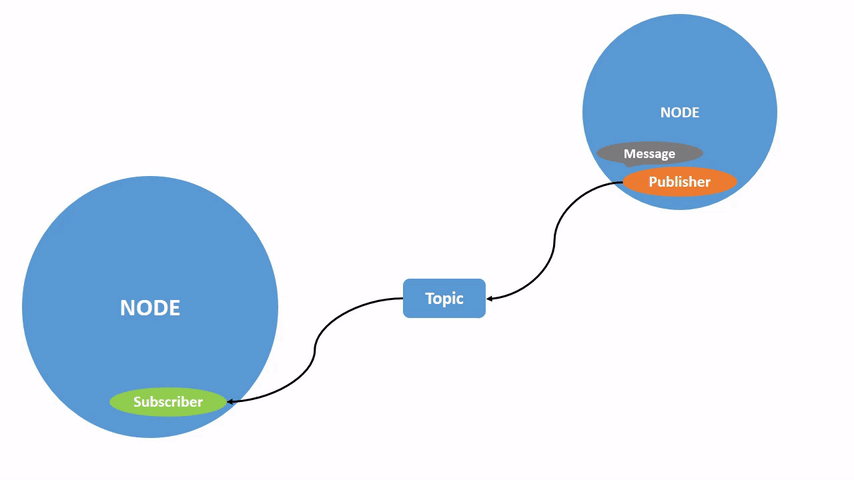
\includegraphics[width=8cm]{img/topicsExplanation.png}
	\caption{Vizualizácia témy v~ROSe~\cite{RosDoc}} \label{fig:topics} \end{figure}

\newpage
\subsubsection{Služby}

\textbf {Služby} sú sprostredkované pomocou TCP/IP protokolu. Poskytujú nám rovnaký spôsob komunikácie ako témy, až na~to, že sa správy
medzi servisom a~klientom posielajú cez LAN (\acrlong{LAN}) a oboma smermi. Služby sa využívajú pri komunikácii medzi viacerými zariadeniami.

\begin{figure}[h]
	\centering
	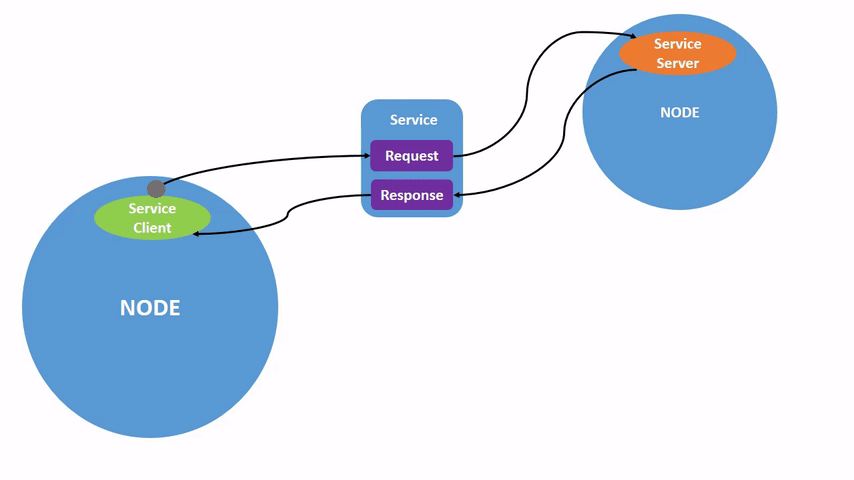
\includegraphics[width=8cm]{img/serviceExplanation.png}
	\caption{Vizualizácia služby v~ROSe~\cite{RosDoc}}
	\label{fig:service}
\end{figure}

\subsubsection{Akcie}

\label{s_action}
\textbf {Akcie} (TCP/IP) sú najzložitejším spôsobom komunikácie. Tento spôsob bol pridaný do~ROS1 až neskôr. V~druhej verzii ROSu je tento
typ komunikácie medzi troma základnými. Sú založené na~službách a prebiehajú asynchrónne~\cite{ROS2book} a~máju 3 stavy. Najprv pošle klient serveru,
akú akciu má vykonať, server mu potvrdí, že túto požiadavku dostal. Server začne následne vykonávať danú akciu a~posielať klientovi priebežné správy
o~priebehu vykonávania žiadanej úlohy. Keď server skončí pošle klientovi výsledok akcie a~klient mu obratom potvrdí obdržanie výsledku.

\begin{figure}[h]
	\centering
	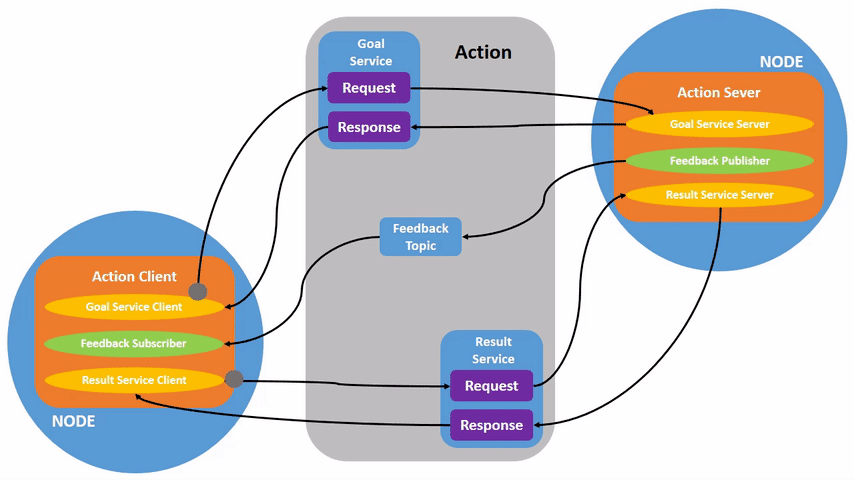
\includegraphics[width=8cm]{img/actionExplanation.png}
	\caption{Vizualizácia akcie v~ROSe~\cite{RosDoc}}
	\label{fig:action}
\end{figure}

\subsection{Parametre}

\label{s_parametre}
\textbf{Parametre} sú spôsob, ako môže komunikovať užívateľ so základnými nastaveniami programu bez potreby zmenenia kódu a jeho následnej kompilácie.
Definujú sa v~\textit{yaml} konfiguračnom súbore. V~ňom si môžeme zadefinovať mená jednotlivých parametrov a ich základné hodnoty. Tie si vieme v~programe
vytiahnuť pomocou API, \acrlong{API}, (Aplikačné Programovacie Rozhranie) v~ROSe.

\begin{figure}[!htbp]
	\centering
	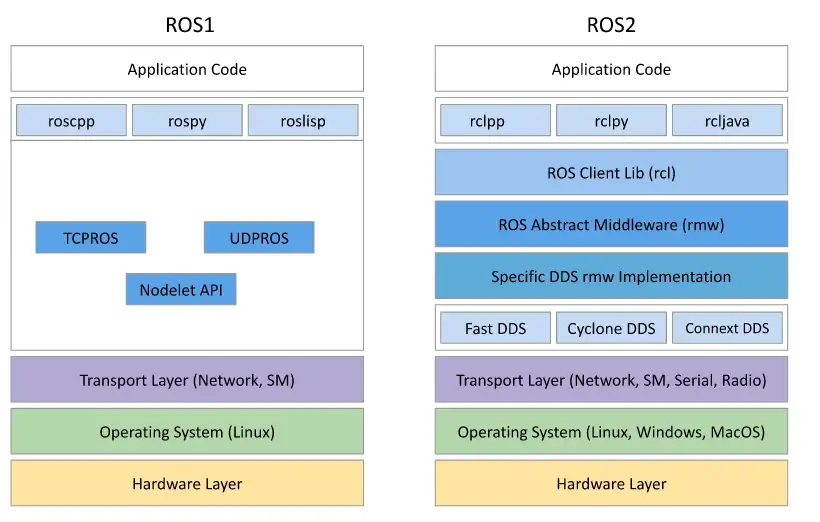
\includegraphics[width=15cm]{img/strukturaRos1Ros2.png}
	\caption{Porovnanie štruktúr ROS1 a~ROS2~\cite{comparison}}
	\label{fig:struktury}
\end{figure}

\subsection{ROS1}

\noindent ROS bol prvýkrát vydaný v~roku 2007. Ide o~softvér, ktorý sa začal vyvíjať so zámerom zjednodušiť programovanie a~ovládanie robotov. Od doby,
kedy vznikol prešiel mnohými verziami a~úpravami. Jeho neoddeliteľnou súčasťou sú štrukturovanie programu do~uzlov (nodov), komunikácia medzi uzlami,
podpora viacerých programovacích jazykov ako sú C, C++ alebo Python a~vytváranie balíčkov dostupných širokej verejnosti.

Štrukturalizovanie základov ROS1 je spravené monoliticky čo najstabilnejším spôsobom. Na~počiatku programu musíme spustiť hlavný program (roscore),
ktorý zabezpečuje vytváranie jednotlivých uzlov. Komunikácia medzi uzlami je zabezpečená prostredníctvom prepojenia uzlov cez LAN/WLAN alebo IPC komunikáciu.
Ak sú uzly spustené na~iných zariadeniach, tak sa využíva len komunikácia cez sieť. Roscore ďalej poskytuje parametre jednotlivým uzlom z~parametrového
servera. Jeho najväčšou úlohou je zabezpečenie komunikácie uzlov v~programe.

\pagebreak

Aj napriek mnohým výhodám má ROS1 aj nedostatky, ktoré sa ťahajú už od~jeho počiatkov. Sú to~napríklad:
\begin{itemize}
	\item Nepostačujúca distribuovanosť systému. Ak prestane fungovať roscore, prestane ísť celý program,
	\item ROS1 je písaný v~starom štandarde, to~vnáša do~programu technologický dlh a~bezpečnostné riziká,
	\item Kvalita komunikácie sa nedá ovplyvniť
	\item Jedno vláknový komunikačný model spomaľuje systém
\end{itemize}

Kvôli takýmto problémom sa začala vyvíjať nová verzia ROSu, ROS2. Tá mala vyriešiť tieto problémy a~zlepšiť funkcionalitu prvej verzie. V~roku 2025 sa skončí
podpora poslednej distribúcie ROS1 menom \textit{Noetic}. Preto~je odporúčané začínať nové projekty v~ROS2.

\subsection{ROS2}

Ako už bolo spomenuté zámerom vývoja ROS2 je zlepšenie funkcionality a~bezpečnosti systému. ROS2 nie je spätne kompatibilný.
Podstata toho, ako sú zoskupované uzly a~ako spolu komunikujú je diametrálne odlišná od~ROS1. Z~tohto dôvodu bol vyvinutý takzvaný rosbridge,
ktorý zabezpečuje kompatibilitu medzi verziami. Nie je to~ale trvalé riešenie. Odporúčané je nástroj využívať a~počas toho prepisovať kód
z verzie 1 do~verzie 2. Komunikácia prebieha \newline v~ROS2 rovnakým spôsobom ako v~ROS1. Pomocou tém, služieb a~akcií.

Táto podobnosť končí na~najvyššej vrstve. Ako sme videli na~Obr.~\ref{fig:struktury}. Štruktúra ROS2 je rozdelená do~viacerých vrstiev.
Najdôležitejšie je pre~nás vedieť, že komunikácia je spracovávaná modelom DDS (Služba distribúcie údajov) z~anglického (\acrlong{DDS}). Tento model zlepšuje výkon, stabilitu
a bezpečnosť modelu oproti ROS1. Je založený na~TCP/UDP protokole. Z~obrázku vyčítame aj lepšie rozloženie modulov. To~zabezpečuje jednoduchšie
prispôsobovanie systému pre~nové funkcionality. Podpora operačných systémov sa v~ROS2 rozšírila aj o~Windows, Mac OS či~operačné systémy reálneho času.
Operačne systémy nie sú jediné rozšírenie ohľadom kompatibility. S ROS2 je možné programovať už aj v~Jave či~Matlabe.
Tvorcovia mysleli aj na~programátorov a~pridali rozšírené možnosti testovania, debugovania či~nasadzovania programu do~reálneho využitia.

ROS2 ma necentralizovanú štruktúru, a~preto pri spúšťaní programov už nie je potrebné mať spustený roscore. Ak teda spadne
jeden proces druhé budú fungovať naďalej. V~ROS1 sme vedeli ovplyvniť počet uchovaných správ pokým nepretiekol zásobník, ktorý ich uchovával na~neskoršie použitie.
V ROS2 vieme zmeniť kvalitu komunikácie. Vieme si zadefinovať, či~by sme radšej stratili niektoré správy, ale dostali by sme všetky rýchlo. Alebo aby sa zabezpečilo,
že dostaneme všetky správy, ktoré boli vyslané, aj keby to~trvalo dlhšie. Dokonca si vieme zadefinovať maximálny čas, ktorý budeme čakať na~ďalšiu správu.

Pri všetkých týchto zlepšeniach nemôžeme zabudnúť aj nasledovný nedostatok. Keďže ROS2 je mladší ako ROS1 nájdeme k nemu menej dokumentácie.
Pridaním veľkého počtu funkcionalít začal vznikať problém pre~začiatočníkov s~porozumením niektorých kódov. Avšak tento problém je nedostatkom,
ktorý časom zanikne. V~čase písania tejto prace pribudli na~stránke dokumentácie 2 strany popisujúce pokročilejšie Funkcionality druhej verzie ROSu.

\subsection{Rozdiely}

Čo je určite dobrou správou pre~všetkých programátorov, ktorí robili v~prvej verzii a~sú zvyknutí na~jej štandardy a~funkcionalitu sa nemajú čoho obávať.
Prechod z~ROS1 na~ROS2 je dosť priamočiary. Čo sa zmenilo je spôsob písania kódu, ale koncepty funkcionality ostali všetky rovnaké. V~tejto sekcii nebudeme
písať konkrétne kódy, budeme len opisovať čo je podobné a~čo zasa rozdielne medzi verziami spomínaného systému. Keďže celý projekt bol písaný v~programovacom
jazyku C++ tak sa aj tieto zmeny budu týkať hlavne C++.

\subsubsection{Štandard jazyka}

	Pokým ROS1 bola písaná v~štandarde C++98 tak ROS2 je už písaná v~novom štandarde. To~zahŕňa inicializovanie templatov a~ich použivanie. Definície
	a deklarácie templatov sú na~knihu samú o~sebe, preto do~detailov nebudeme zachádzať. Stačí nám vedieť, ako ich inicializovať. V~prvej verzii
	sme definovali publishera (publikovateľa) všeobecného a~definovali sme mu cez aký topic má posielať správy. V~druhej verzii naväzujeme publishera
	na špecifický tip správy akú posielame. Nemôže sa teda stať, že takýto program by sme skompilovali a~následne keď ho spustíme tak by spadol.

\subsubsection{Inicializácia nody(uzla)}

	Tak isto ako v~prvej verzii aj v~druhej verzii musíme definovať nodu. Rozdiel je v~tom, že prvá verzia obsahovala NodeHandle a~druha verzia obsahuje priamo Node.
	V druhej verzii je zaužívaným štandardom tuto nodu precediť a~použiť polymorfizmus pri objekte, ktorý musí existovať počas celej doby vykonávania programu. Pri
	prvej verzii tomu tak nebolo. Museli sme vytvoriť už spomenutý NodeHandle. Ten sa nemusel využiť ako base trieda a~nemusel ani~existovať počas celého behu programu.

\newpage
\subsubsection{Komunikácia}

	DDS (Služba distribúcie údajov) je protokol strednej vrstvy (middleware) implementovaný nad UDP~\cite{ROS2book}. Je používaný v~ROS2 na~komunikáciu
	medzi uzlami. Je to~systém správ publikovania (publish) / odoberania (subscribe), ktorý umožňuje uzlom komunikovať medzi sebou bez toho,
	aby poznali identitu ostatných uzlov. Druh komunikácie je v~ROS2 rozšírený ešte o~akcie~\ref{s_action}.

\subsection{Parametre}

	ROS1 používa parametrový server, ktorý sa nachádza v~roscore-e. Každý uzol si mohol vytiahnuť parametre, ktoré boli zapísané v~konfiguračnom súbore.
	ROS2 žiadny roscore nemá, preto sa parametre musia distribuovať iným spôsobom. Parametre v~druhej verzii ROSu patria jednotlivým uzlom. To~znamená, že jednotlivé
	parametre sa dajú vytiahnuť len daným uzlom. Tieto parametre taktiež existujú len počas existencie daného uzlu. Parametre si ďalej distribuované pomocou už spomínaného
	DDS protokolu.

\subsubsection{Nodelet alebo komponent}

	ROS1 ponúka možnosť definície uzlov ako \texttt{nodlet}. Je to~definovanie uzlu ako zdielanej knižnice (shared library). Je to~spôsob ako uľahčiť
	prácu CPU. Keď sa definuje zdielaná knižnica tak jeden proces môže spracovávať programy z~viacerých uzlov. Táto funkcionalita sa nachádza aj v~ROS2.
	Volá sa komponent (\texttt{component}). Vylepšením oproti nodeletom je zjednotenie aplikačnej implementácie. Pokým nodelety mali vlastný spôsob
	implementácie v~ROS1 tak v~ROS2 je implementácia uzla a~komponentu rovnaká. Pri~komponente sa musí len naviac definovať, že daný komponent existuje.
	Použitie komponentov zjednodušuje prácu CPU a~používa sa hlavne v~zariadeniach, ktoré majú obmedzený výkon výpočtovej techniky.

\subsubsection{Kompilácia}

	Zmenou verzii sa zmenil aj spôsob kompilácie programu. ROS1 bol kompilovaný pomocou \texttt{catkin} build systému. Catkin je založený na~programe
	\texttt{cmake}. Jeho nastavenie dependencií je konfigurované pomocou súboru \texttt{package.xml} . ROS2 prešiel na~viac nastaviteľný systém \texttt{Colcon}.
	Tento systém je na~rozdiel od~catkinu založený na~Pythone a~jeho dependencie sa nastavujú pomocou \texttt{setup.py} súboru. V~prípade colconu si môžeme
	definovať spôsob kompilácie to~znamena, ze môžeme nastaviť, ako sa budú spracovávať dependencie. Ponúkané možnosti sú \texttt{catkin\_make},
	\texttt{catkin\_make\_isolated}, \texttt{catkin\_tools} a~\texttt{ament\_cmake}. Jednou s~najviac používaných možností je \texttt{ament\_cmake}.
	Je založený na~programe \texttt{cmake} a~spolupracuje so systemom \texttt{colcon}. Z~tohto dôvodu mu vieme mu definovať dependencie pomocou xml
	súboru ako v~ROS1 pričom možnosť definície pomocou python skriptu ostáva. Je to~jeden zo spôsobov, ako zmenšiť rozdiel medzi ROS1 a~ROS2.

\section{Robot}

Robot, s~ktorým sme pracovali bol výsledkom tímového projektu viacerých študentov \newline z~roku 2019. Pri~vysvetľovaní a~opisovaní robota sa budeme odvolávať
na dokumenty, stránky a~kód, ktorý napísali. Všetky tieto údaje si sprístupnené na~mobilnom robote v~záložke
\newline \texttt{\$(HOME)/Desktop/Blackmetal}~\cite{timovyProjekt}.

Robot je v~tvare kvádra. Jeho šírka je 60cm a~je vyzdvihnutý nad zem o~1.5cm. Nachádza sa na~kolesách o~polomere 8cm. Jeho kostra, až na~oceľové pláty, ktoré držia robot,
je spravená z~hliníku. Konkrétne z~hliníkových tyčí, ktoré sú pospájané plexisklovými plátmi. Jeho podobizeň vidíme na~nasledujúcom obrázku. 

\begin{figure}[!htbp]
	\begin{center}
		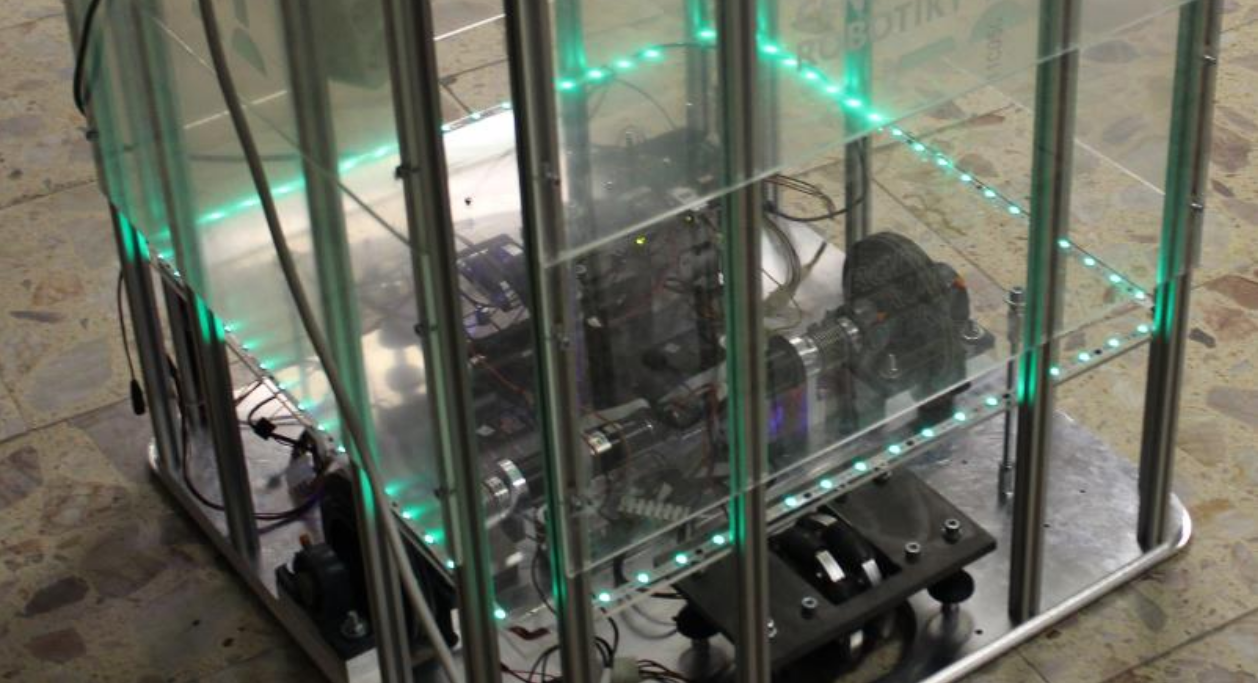
\includegraphics[width=0.95\textwidth]{img/robot.png}
	\end{center}
	\caption{Zobrazenie spodnej časti mobilného robota~\cite{timovyProjekt}}
	\label{fig:robot}
\end{figure}

\noindent Na~obrázku ďalej vidíme olemovanie robota pasom s~LEDkami. Tie svietia nasledovným spôsobom. Keď sa robot nehýbe všetky LEDky svietia
na zeleno. Keď sa robot pohne do~nejakej strany, LEDky znázornia jeho pohyb tým, že svietia na~strane, do~ktorej sa robot hýbe. Keď nastane
situácia, kedy počítač ovládajúci motory prestane komunikovať s~Arduinom, ktoré sa stará o~detekciu stavov robota tak LEDky začnú blikať červeno-modrými farbami.

Ako bolo spomenuté LEDky znázorňujú pohyb robota. Ten sa pohybuje za pomoci diferenciálneho podvozku s~dvoma podpornými všesmerovými kolesami. Motory robota
sú pripojené na~meniče. Tie sú ovládané priamo príkazmi z~počítača.

\subsection{Hardware}

Hardware robota sa skladá z
\begin{itemize}
	\item kontrolnej dosky Arduino Uno,

	\item Počítača ADVANTECH MIO-5272~\cite{robotPc} \newline
		Počítač obsahuje operačný systém Ubuntu.

	\item Extension board MIOe-210~\cite{extensionModule}

	\item Meniče MAXON EPOS 24/5 (s číslom 275512)~\cite{menic} \newline
	 	Sú napájané jednosmerným napätím 11 - 24 V~a~5 A.

	\item Enkódery MAXON Encoder MR Type L (s číslom 225787)~\cite{encoder} \newline
		Rozlíšenie enkóderov je 1024 impulzov s~troma kanálmi.

	\item Motory MAXON RE 40 (s číslom 148867)~\cite{motor} \newline
		Motory s~výkonom 150W. Maximálna rýchlosť je 12 000 rpm a~efektivita 91\%.

	\item Prevodovka MAXON Planetary Gearhead GP 42 C (s číslom 202120)~\cite{prevodovka} \newline
		Redukcia prevodovky je 43:1. Jej účinnosť je 72\%.
\end{itemize}

\noindent Ovládanie robota je zabezpečené externými počítačmi
\begin{itemize}
	\item Control PC (Kontrolný počítač) -- Počítač posielajúci príkazy na~robot cez TCP/IP protokol.
	\item Logging PC (Logovací počítač) -- Počítač prijímajúci stav robota cez TCP/IP protokol.
\end{itemize}

\begin{figure}[!htbp]
	\begin{center}
		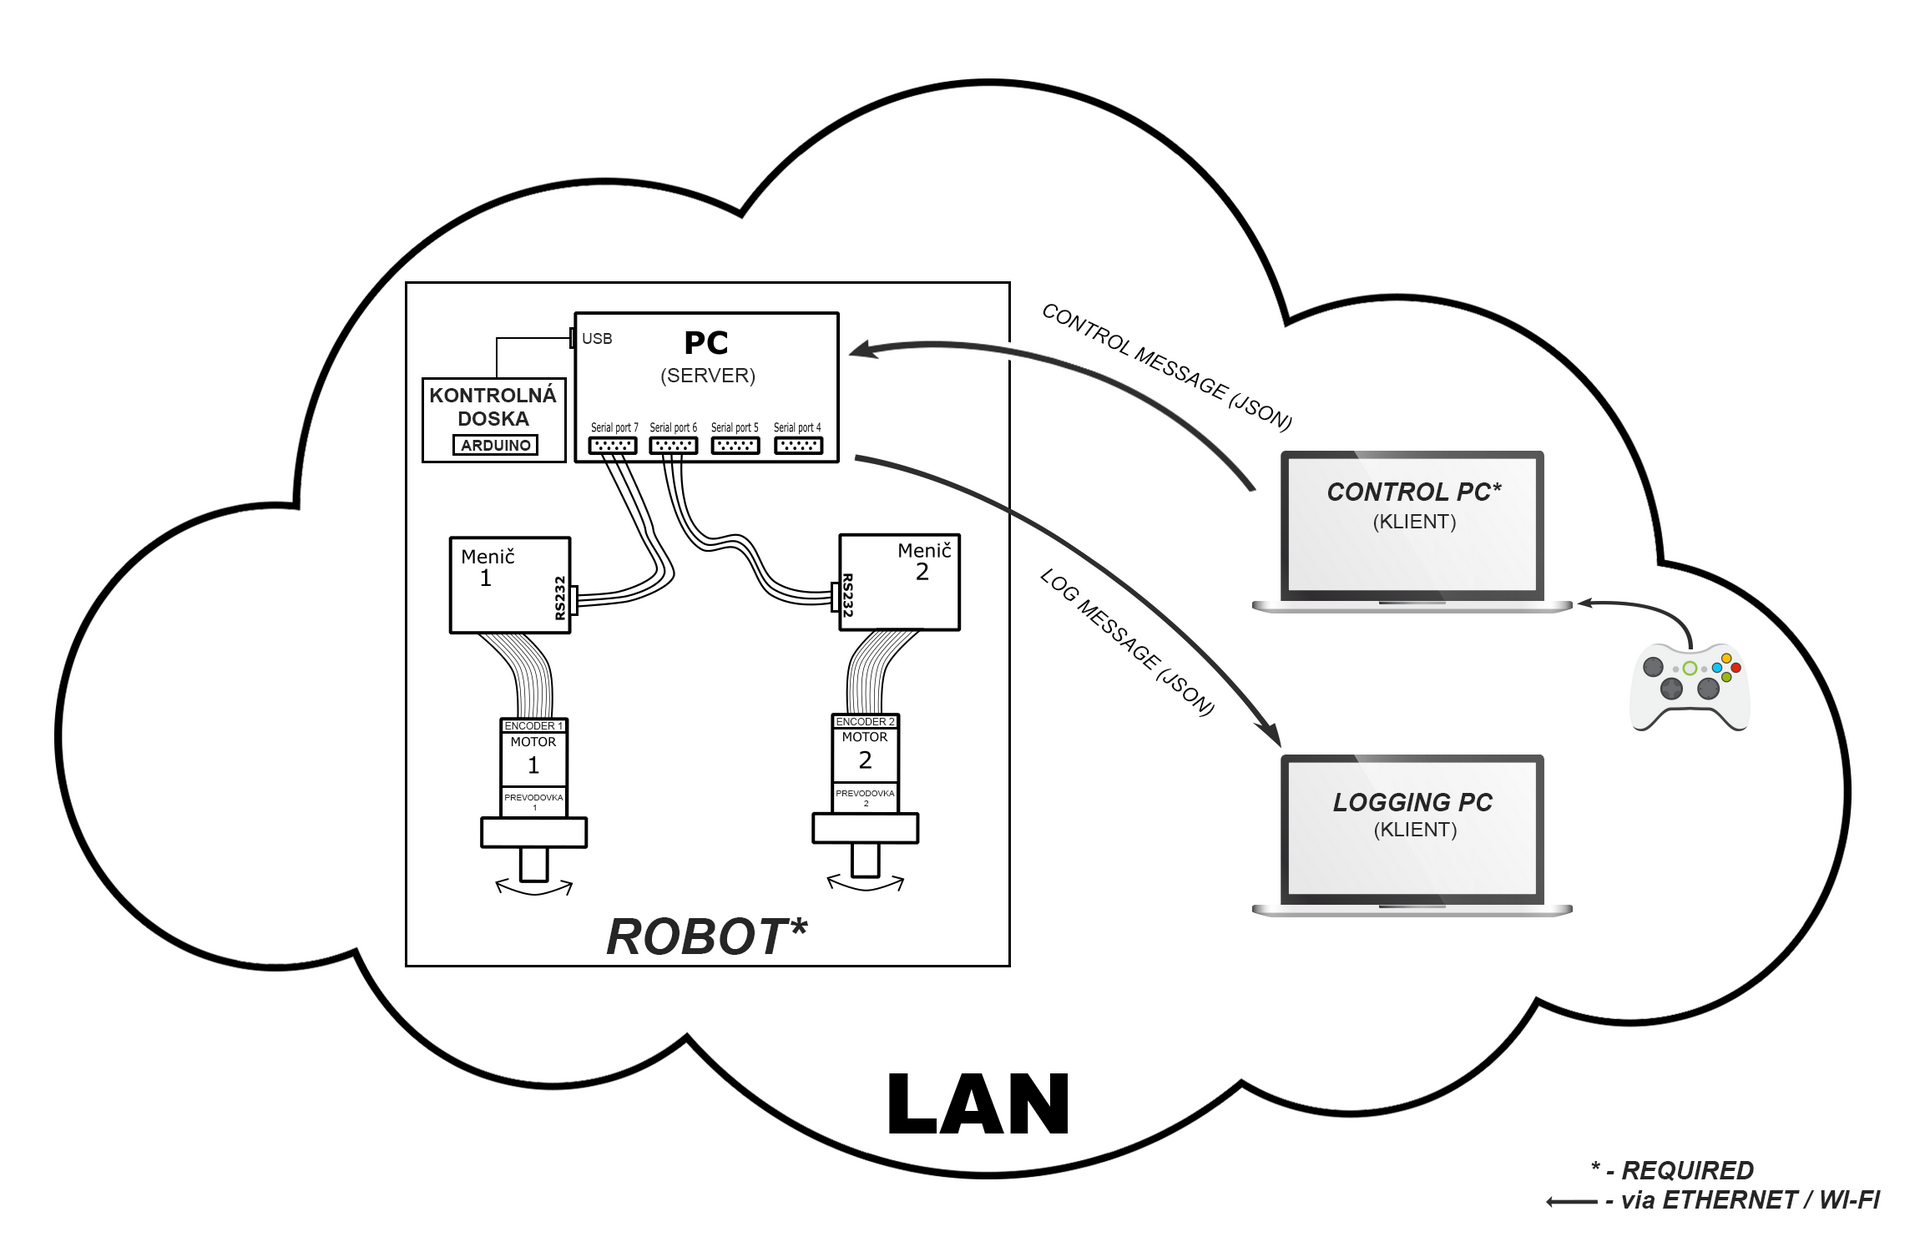
\includegraphics[width=9cm]{img/schemaRobota.png}
	\end{center}
	\caption{Schéma zapojenia jednotlivých častí na~robote}
	\label{fig:schemaRobota}
\end{figure}

Na obrázku Obr.~\ref{fig:schemaRobota} vidíme zapojenie jednotlivých častí robota. Čo sme nespomenuli a~je na~obrázku je XBox ovládač je to~kvôli tomu, že
tímový projekt bol zameraný na~ovládanie robota pomocou tohto ovládača.

\subsection{Komunikácia s~robotom}

S robotom sa vieme spojiť pomocou dvoch portov. Jeden port je otvorený na~prijímanie požiadavok (requestov) a~ten druhy je na~monitorovanie stavu robota. 
Port \textit{664} je otvorený pre~tisíc užívateľov, ktorí môžu len sledovať stav robota. Druhy port je na~prijímanie requestov \textit{665} a~je otvorený
len pre~jedného užívateľa.

\subsubsection{Logovanie}

Spomínaný port \textit{664} je otvorený jednému užívateľovi. Keď sa užívateľ pripojí začne dostavať nepretržite správy typu JSON, ktoré hlásia stav robota. Spravy,
ktoré dostávame sú nasledujúceho formátu
\begin{lstlisting}
		{"state":1,"direction":1}
\end{lstlisting}
Hodnoty sa pri stave (state) a~ani pri smere (direction) nemenia. Sú to~stále jednotky. Pokým robota nezastavíme buď príkazom, alebo stlačením tlačidla vypnutia,
tak sa tieto správy budú posielať. Môžeme potom začať polemizovať o~tom či~by nebolo lepšie už tieto správy využiť na~to~čo reálne spomenutý JSON reťazec ukazuje.

\subsubsection{Ovládanie}

Port \textit{665} je sprístupnený na~prijímanie a~odosielanie požiadavok a~ich odpovedí. Príkazy sa na~počítač posielajú cez sieť z~externého počítača vo formáte
\textbf{JSON}. Študenti, ktorí navrhovali systém posielania požiadavok (request) a~odpovedí (response) robili tieto správy ručne. Preto~nastávajú situácie, kedy
robot pošle správu, ktorá nespadá do~štandardu písania JSON textu. Z~tohto dôvodu sme nemohli použiť už existujúci kód, ktorý by nám zjednodušil prehľadávanie
týchto sprav. Podla dokumentácie sa robot mal ovládať správami typu~\cite{BMdoc}

\label{jsonSpeedRequestBad}
\begin{lstlisting}
		{"UserID":1,"Command":3,"RightWheelSpeed":50,"LeftWheelSpeed":50}
\end{lstlisting}

\newpage

\noindent Význam jednotlivých parametrov:
\begin{itemize}
	\item \textbf{UserID} -- Znázorňuje ID užívateľa, ktorý je pripojený na~robot. Predvolená hodnota je 1.
	\item \textbf{Command} --  Číselná hodnota znázorňujúca príkaz, ktorý ma robot vykonať
		\begin{enumerate}
			\setcounter{enumi}{-1}
			\item \label{c0} Prázdny príkaz slúžiaci na~overenie spojenia
			\item \label{c1} Núdzové zastavenie
			\item \label{c2} Normálne zastavenie
			\item \label{c3} Príkaz nastavujúc rýchlosti kolies mobilného robota
			\item \label{c4} Prázdny príkaz
			\item \label{c5} Prázdny príkaz
			\item \label{c6} Príkaz pýtajúci si aktuálnu rýchlosti pravého a~ľavého kolesa. Tento príkaz nebol sprave navrhnutý v~kóde robota. Vracal nám žiadaná hodnotu
				namiesto aktuálnej. Museli sme ho prepísať
			\item \label{c7} Pripravenie motorov robota
			\item \label{c8} Príkaz pýtajúci si aktuálnu pozíciu pravého a~ľavého kolesa.
		\end{enumerate}
	\item \textbf{RightWheelSpeed} -- Nastavenie rýchlosti pre~pravé koleso
	\item \textbf{LeftWheelSpeed} -- Nastavenie rýchlosti pre~ľavé koleso
\end{itemize}

\noindent Z~tohto kusu kódu je jasné, že sa majú posielať celé čísla a~na základe tohto vstupu sa bude robot hýbať. Čo sme zistili až po skompilovaní
a spustení tímového projektu je, že sa majú posielať desatinné čísla z~intervalu 0 až 1. Po spomenutí tejto skutočnosti môžeme uviesť vyznám jednotlivých parametrov.
Toto bolo písané v~dokumentácii, ktorá nám bola dodaná na~začiatku programu. Môžeme preto príklad prepísať na~reťazec, ktorý by fungoval

\label{jsonSpeedRequestGood}
\begin{lstlisting}
		{"UserID":1,"Command":3,"RightWheelSpeed":0.50,"LeftWheelSpeed":0.50}
\end{lstlisting}

\subsection{Par slov k parametrom reťazca}

\noindent \textbf{UserID} \newline
\indent Táto možnosť je v~momentálnom stave robota nevyužitá. Počet zariadení, ktoré sa môžu pripojiť na~port, cez ktorý sa dá robot ovládať je 1. Je to~ale
dobrá možnosť na~rozšírenie kódu. Keď sa budú môcť pripojiť viacerí užívatelia, tak sa bude musieť vyriešiť, koho príkaz bude mať akú prioritu. \newline

\noindent \textbf{Command:4} \newline
\indent Tento príkaz je prázdny. My sme ho ale neskôr prepísali na~príkaz, cez ktorý sa dá nastaviť žiadaná pozícia kolies robota (natočenie). Táto funkcionalita nie je
v takom stave ako sme si priali. \newline

\noindent \textbf{RightWheelSpeed/LeftWheelSpeed} \newline
\noindent Nastavovanie rýchlosti pravého a~ľavého kolesa nie sú povinne parametre. Musíme ich zadávať len v~prípade posielania rýchlostí cez príkaz s~číslom \ref{c3}.

\section{Oprava chýb na~robote}

\subsection{Nesprávna funkcia}
\indent Ako bolo spomenuté vyššie, pri poslaní príkazu s~číslom \ref{c6} nám robot vráti aktuálne rýchlosti kolies. Počas skúšaní tejto funkcionality sme narazili na~problém.
Keď sme sa robota spýtali na~jeho rýchlosti dostali sme reťazec, ktorý obsahoval náhodne veľké čísla. Tieto čísla za menili keď sme zadávali nejaké hodnoty pre~rýchlosti kolies
aby sa robot hýbal.

\label{jsonWannabeSpeed}
\begin{lstlisting}
		{"LeftWheelSpeed"=236223201280 "RightWheelSpeed"=4294967296}
\end{lstlisting}

Tu vidíme príklad obdržanej spravy. Ako si môžeme všimnúť. Pri~tomto type správ nie je dodržaná správna forma reťazca typu JSON. Namiesto `:' máme `='
a medzi argumentmi sa nenachádza čiarka. Jeden z~nápadov, ktorý sme mali bolo premeniť tieto čísla na~desatinné čísla, keďže sme mu posielali taký formát čísel.
Problém je v~tom, že keď posielame request na~nastavenie rýchlosti kolies, tak kód na~robote funguje tak, že si ich premení na~celé čísla v~rozsahu 0 až 1000.
To~je hodnota, na~ktorú nastaví rýchlosti otáčania kolies, rýchlosť otáčania motora. Na~druhú stranu, keď si vypýtame od~robota rýchlosti kolies. On zoberie
informáciu z~enkóderov a pošle nám to~bez spracovania.

Po dôkladnom preštudovaní kódu sme zistili, že hodnoty ktoré nám posiela nie sú ani~vyťahované z~enkóderov správnou funkciou. Preto~sme ju zmenili a~začali sme dostávať hodnoty,
s~ktorými by sa mohlo dať pracovať.

Funkcie z~knižnice zabezpečujúce komunikáciu z~enkóderov motorov pochádzajú z~firmy Maxon~\cite{EPOSdoc}. Funkcie, ktoré končia koncovkou `Target' majú
návratné hodnoty reprezentujúce žiadané hodnoty. Funkcie s~koncovkou `Is' vracajú aktuálne hodnoty. Z~tohto dôvodu sme museli prepísať funkciu, ktorá sa vykonávala,
keď sme chceli získať aktuálne hodnoty rýchlosti motora poslaním príkazu \ref{c6}.

\lstset{language=C++,
	basicstyle=\ttfamily,
	keywordstyle=\color{blue}\ttfamily,
	stringstyle=\color{red}\ttfamily,
	commentstyle=\color{green}\ttfamily,
	morecomment=[l][\color{magenta}]{\#},
	numberstyle=\color{orange}
}

\label{VelocityIs}
\begin{lstlisting}[language=C++]
BOOL VCS_GetTargetVelocity(
	HANDLE KeyHandle,
	WORD NodeId,
	long* pTargetVelocity,
	DWORD* pErrorCode);
\end{lstlisting}

\begin{lstlisting}[language=C++]
BOOL VCS_GetVelocityIs(
	HANDLE KeyHandle,
	WORD NodeId,
	long* pVelocityIs,
	DWORD* pErrorCode);
\end{lstlisting}

\noindent Ako môžeme vidieť v~týchto predpisoch funkcií, bolo treba zmeniť názov funkcie a~ostatné parametre ostali rovnaké.
Nebolo treba meniť implementáciu kódu.

\subsection{Zašumený výstup}

Po~prepísaní funkcie na~získavanie rýchlostí robota sme spravili pár meraní, aby sme zistili, aké presné informácie o~rýchlostiach
motorov dostávame. Aby nám robot neodbiehal postavili sme ho na vyvýšené miesto, tak aby sa kolesá nedotýkali zeme. V~takomto
postavení sa robot nepohne z~miesta a~my môžeme bez~problémov odmerať prechodové a~prenosové charakteristiky rýchlosti pravého
a~ľavého motora.

\begin{figure}[!htbp]
	\begin{center}
		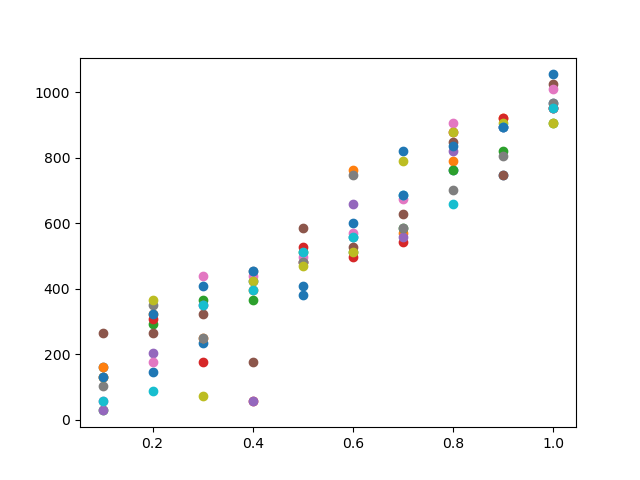
\includegraphics[width=8cm]{img/Left_wheel.png}
	\end{center}
	\caption{Ustálené hodnoty rýchlosti ľavého motora. }
	\label{fig:laveKoleso}
\end{figure}

\begin{figure}[!htbp]
	\begin{center}
		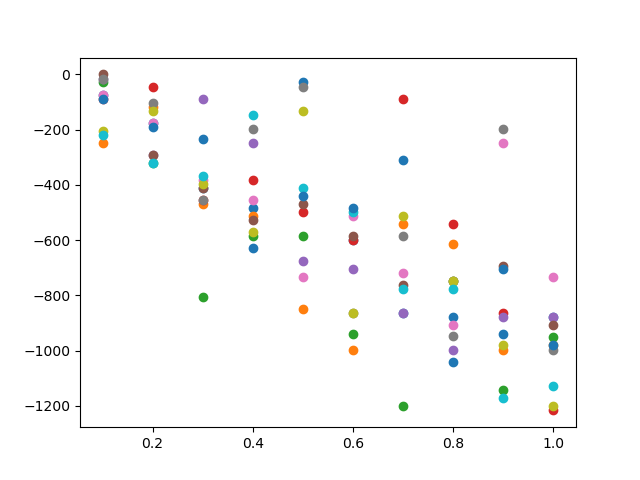
\includegraphics[width=8cm]{img/Right_wheel.png}
	\end{center}
	\caption{Ustálené hodnoty rýchlosti pravého motora. }
	\label{fig:praveKoleso}
\end{figure}

\begin{figure}[!htbp]
	\begin{center}
		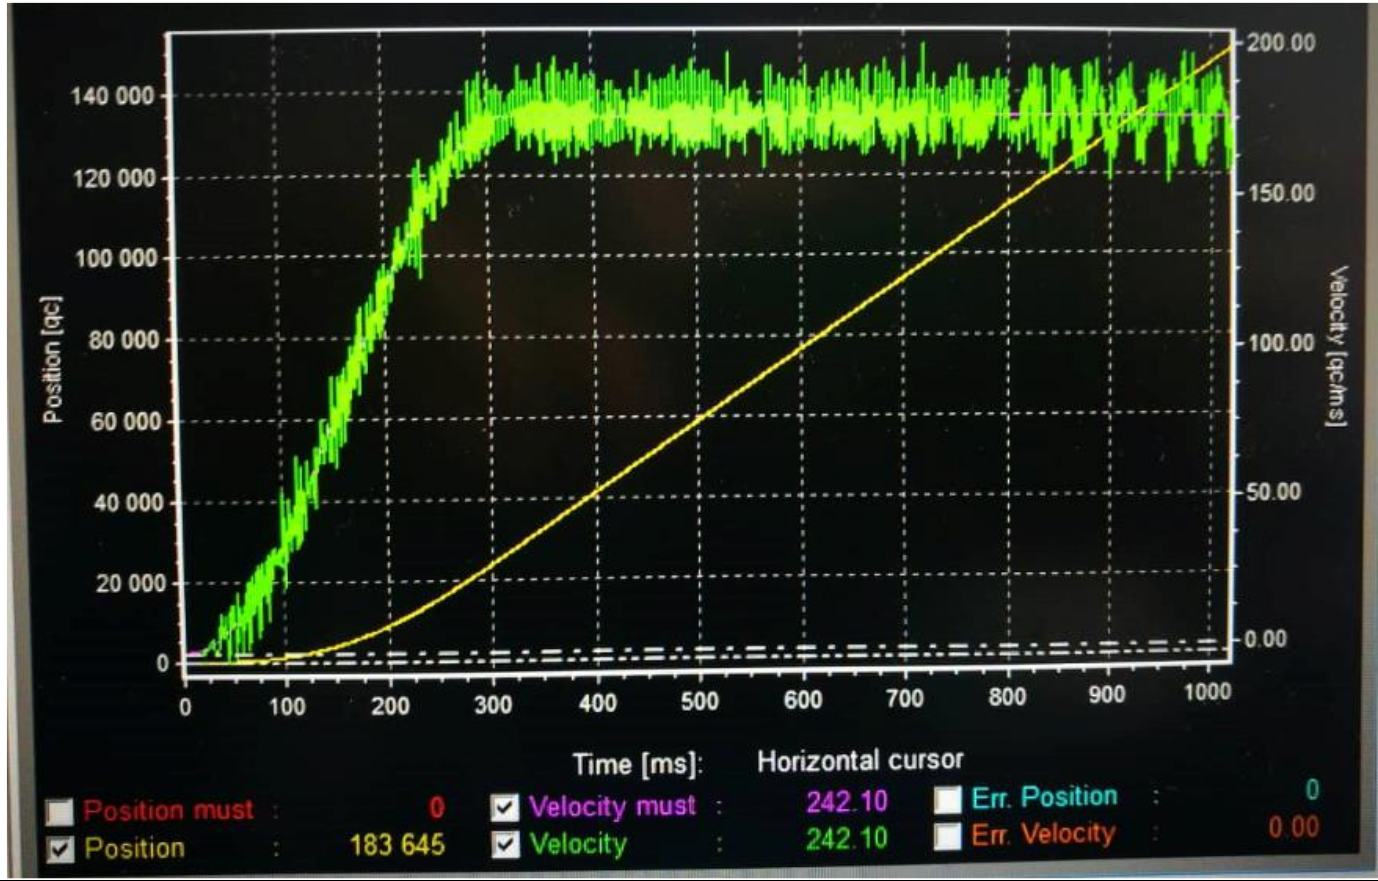
\includegraphics[width=0.95\textwidth]{img/robotSpeedChar.png}
	\end{center}
	\caption{Prechodová charakteristika rýchlosti kolies~\cite{timovyProjekt}. }
	\label{fig:prechChar}
\end{figure}

